\section{1174077 - Alvan Alvanzah}
Chapter 3 - Prediksi dengan Random Forest
\subsection{Teori}
\subsubsection{ Jelaskan apa itu random forest, sertakan gambar ilustrasi buatan sendiri.}
\hfill\\
Random Forest adalah sebuah algoritma yang digunakan terhadap klasifikasi data dalam jumlah yang besar. Klasifikasi pada random forest dilakukan dengan penggabungan dicision tree dengan melakuakn training terhadap sempel data yang dimiliki. Semakin banyak dicision tree maka data yang di dapat akan
semakin akurat.

\begin{figure}[H]
	\centering
	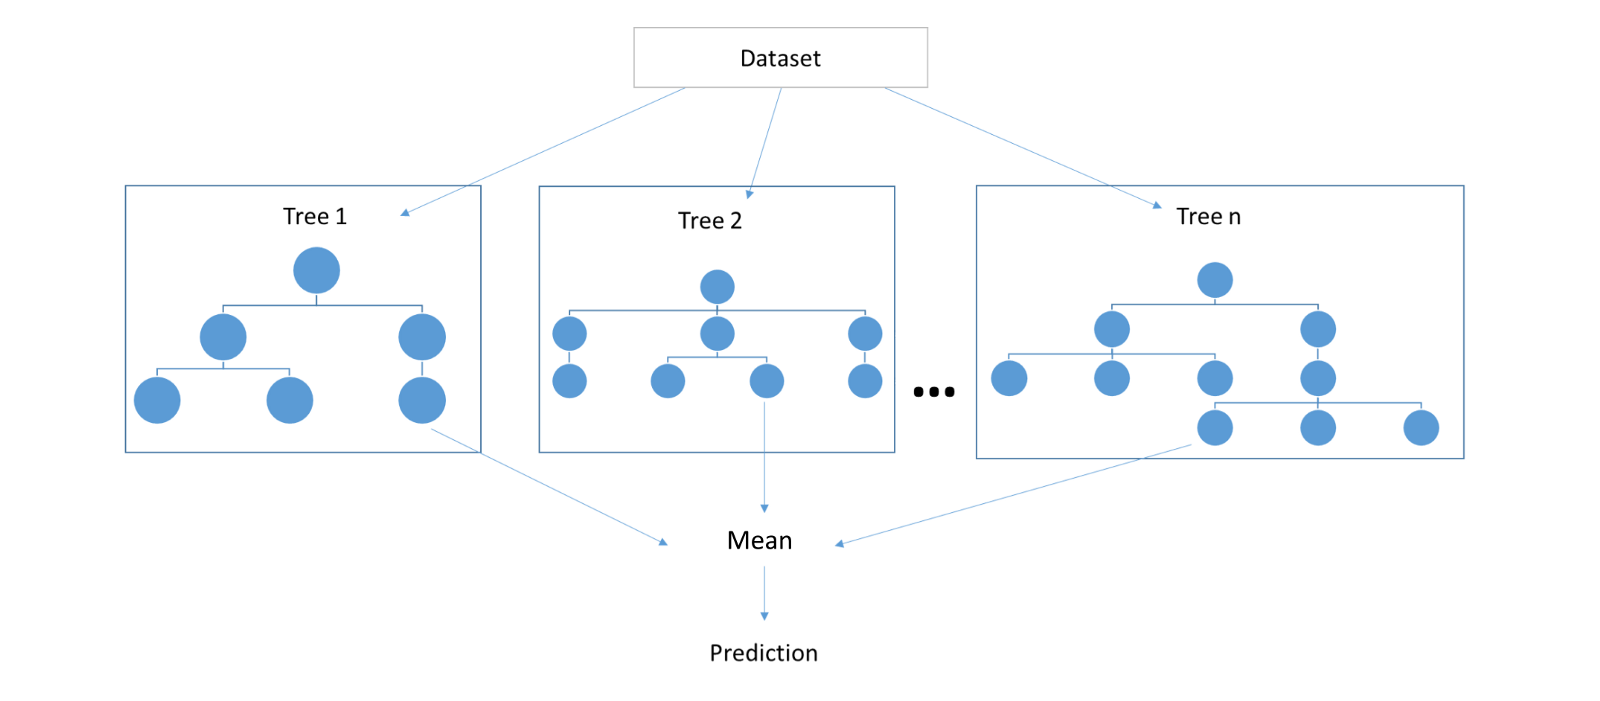
\includegraphics[width=12cm]{figures/1174077/3/1.png}
	\caption{Random forest}
\end{figure}


\subsubsection{Jelaskan cara membaca dataset kasus dan artikan makna setiap file dan isi field masing masing file.}
\hfill\\
\begin{enumerate}
\item cara membaca dataset
\hfill\\
	\begin{itemize}
	\item Gunakan librari Pandas pada python untuk dapat membaca dataset dengan format text file.
	\item Setelah itu,buat variabel baru ”dataset” yang berisikan perintah untuk membaca file csv. seperti berikut
	\hfill\\
	\lstinputlisting[firstline=8, lastline=10]{src/1174077/3/1174077.py}
	Pada kodingan diatas dapat dijelaskan bahwa : Memanggil Librari Panda untuk membaca dataset Membuat variabel ”Dataset” yang berisikan pd.read\_csv untu kmembaca dataset.
	
	\item setelah di run maka hasilnya seperti berikut
	\hfill\\
\begin{figure}[H]
	\centering
	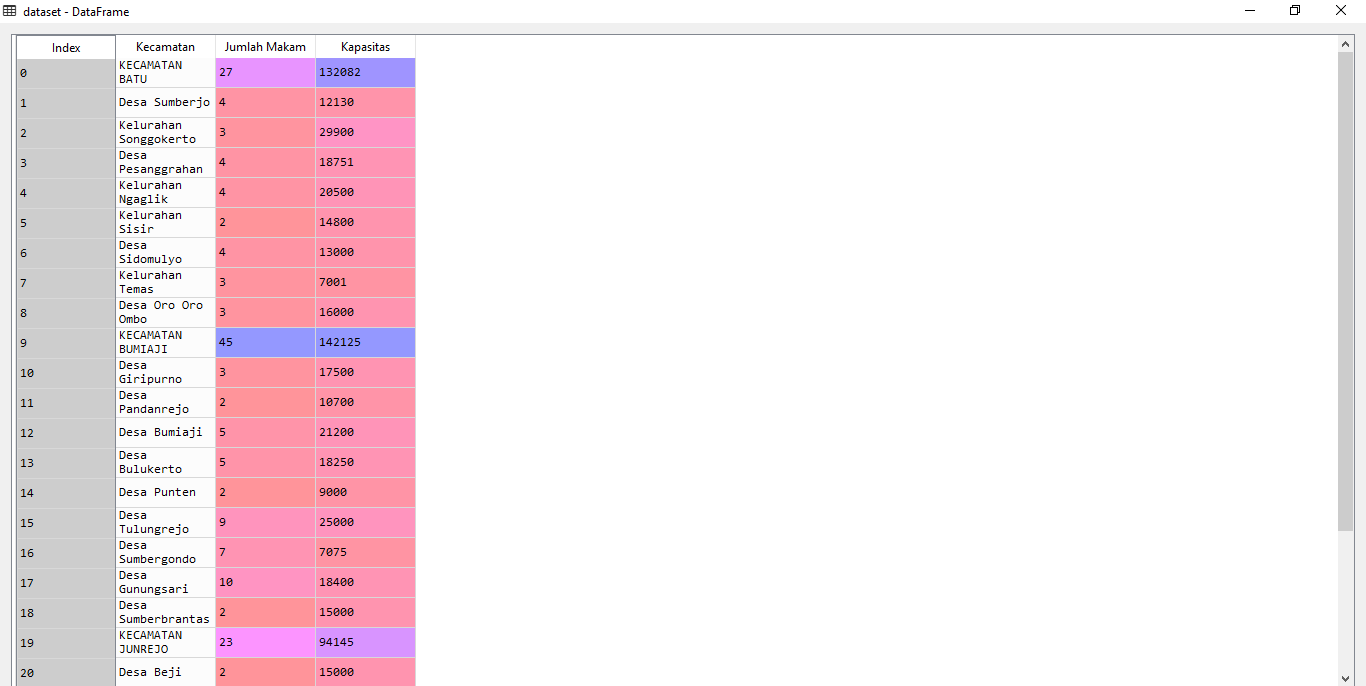
\includegraphics[width=12cm]{figures/1174077/3/2.png}
	\caption{contoh dataset}
\end{figure}
	
	Gambar diatas merupakan dataset Jumlah Tempat Pemakaman Umum (TPU) Kota Batu 2019. Datasetnya didapat dari laman https://data.go.id/dataset/jumlah-tempat-pemakaman-umum-tpu-kota-batu-2019. Penjelasan dari isi field diatas adalah sebagai berikut :
	\begin{itemize}
	\item Atribut Index merupakan atribut otomatis untuk penomoran data yang ada. 
	\item Atribut kecamatan merupakan kecamatan yang ada pada kota batu
	\item Atribut jumlah merupakan jumlah makan yang ada pada kecamatan
	\item Atribut kapasitas merupakan daya tampung pemakaman pada kecamatan
	\end{itemize}
	\end{itemize}
\end{enumerate}

\subsubsection{ Jelaskan apa itu cross validation}
\hfill\\
Cross Validation adalah sebuah teknik validasi model yang berfungsi untuk melakukan penilaian bagaimana hasil analisis statistik akan digeneralisasi ke data yang lebih independen. Cross validation digunakan dengan tujuan prediksi, dan bila kita ingin memperkirakan seberapa akurat model model prediksi yang dilakukan dalam sebuah praktek. Tujuan dari cross validation yaitu untuk mendefinisikan dataset guna menguju dalam fase pelatihan untuk membatasi masalah seperti overfitting dan underfitting serta mendapatkan wawasan tentang bagaimana model akan digeneralisasikan ke set data independen.

\subsubsection{Jelaskan apa arti score 44\% pada random forest, 27\% pada decission tree dan 29\% dari SVM.}
\hfill\\
Dimana Score 44 \% didapatkan dari hasil pengelohan dataset jenis burung. Dimana akan dilakukan proses pembagian data testing dan data training lalu diproses dan menghasilkan score sebanyak 44 \% dimana menjelaskan bahwa score tersebut digunakan sebagai pembanding dalam tingkat keakuratannya. Pada dicision tree akan memperoleh data lebih kecil yaitu sebanyak 27 \% hal ini dikarenakan data yang diolah menggunakan dicision tree dibagi menjadi beberapa tree dan lalu disimpulkan untuk mendapatkan data yang akurat. Pada SVM akan memperoleh score sebanyak 29 \% hal ini dikarenakan data yang dimiliki masih bernilai netral sehingga tingkat keakuratannya masih belum jelas.

\subsubsection{Jelaskan bagaimana cara membaca confusion matriks dan contohnya memakai gambar atau ilustrasi sendiri.}
\hfill\\
Perthitungan Confusion Matriks dapat dilakukan sebagai berikut. Disini saya menggunakan data yang dibuat sendiri untuk menampilkan data aktual dan prediksi.
\begin{itemize}
\item Import librari Pandas, Matplotlib, dan Numpy.
\item Buat variabel y actu yang berisikan data aktual.
\item Buat variabel y pred berisikan data yang akan dijadikan sebagai prediksi.
\item Buat variabel df\_confusion yang berisikan crosstab untuk membangun tabel tabulasi silang yang dapat menunjukkan frekuensi kemunculan kelompok data tertentu.
\item Pada variabel df\_confusion definisikan lagi nama baris yaitu Actual dan kolomnya Predicted
\item Kemudian definisikan suatu fungsi yang diberi nama plot\_confusion\_matrix yang berisikan pendefinisian confusion matrix dan juga akan di plotting. untuk code lengkapnya sebagai berikut:
\lstinputlisting[firstline=14, lastline=32]{src/1174077/3/1174077.py}
\end{itemize}
Hasil dari kode diatas akan menghasilkan confusion matrix seperti berikut:
\begin{figure}[H]
	\centering
	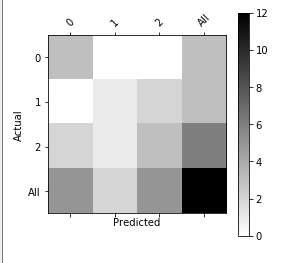
\includegraphics{figures/1174077/3/3.png}
	\caption{hasil confusion matrix}
\end{figure}

\subsubsection{Jelaskan apa itu voting pada random forest disertai dengan ilustrasi gambar sendiri.}
\hfill\\
Voting yaitu suara untuk setiap target yang diprediksi pada saat melakukan Random Forest. Pertimbangkan target prediksi dengan voting tertinggi sebagai prediksi akhir dari algoritma random forest.

\begin{figure}[H]
	\centering
	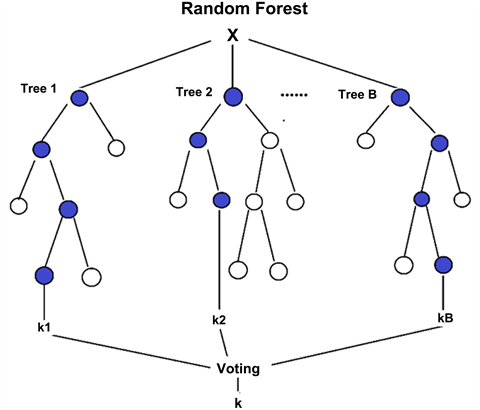
\includegraphics[width=8cm]{figures/1174077/3/4.png}
	\caption{voting random forest}
\end{figure}

\subsection{Praktek}
\subsubsection{Nomor 1}
\hfill\break
\lstinputlisting[firstline=9, lastline=14]{src/1174077/3/Praktek.py}
\begin{figure}[H]
\centerline{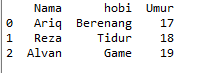
\includegraphics[width=10cm]{figures/1174077/3/5.png}}
\caption{Membuat Aplikasi pakai pandas}
\label{labelgambar}
\end{figure}

\subsubsection{Nomor 2}
\hfill\break
\lstinputlisting[firstline=17, lastline=19]{src/1174077/3/Praktek.py}
\begin{figure}[H]
\centerline{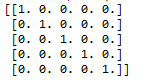
\includegraphics[width=10cm]{figures/1174077/3/6.png}}
\caption{Membuat Aplikasi pakai numpy}
\label{labelgambar}
\end{figure}

\subsubsection{Nomor 3}
\hfill\break
\lstinputlisting[firstline=22, lastline=26]{src/1174077/3/Praktek.py}
\begin{figure}[H]
\centerline{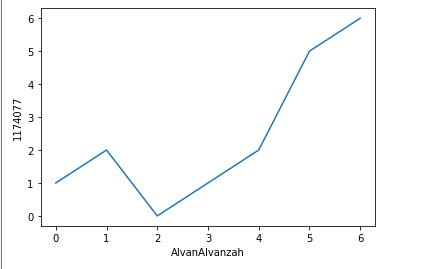
\includegraphics[width=10cm]{figures/1174077/3/7.png}}
\caption{Membuat Aplikasi pakai matplotlib}
\label{labelgambar}
\end{figure}

\subsubsection{Nomor 4}
\hfill\break

\begin{itemize}
\item Source Code pertama pada random forest berfungsi untuk membaca dataset yang memiliki format text file dengan mendefinisikan variabel yang bernama imgatt. Variabel tersebut berisi value untuk membaca data.
\lstinputlisting[firstline=34, lastline=38]{src/1174077/3/Praktek.py}
\begin{figure}[H]
\centerline{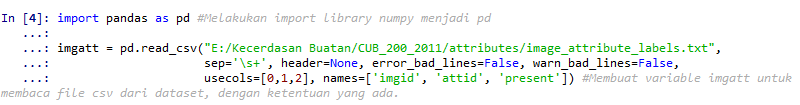
\includegraphics[width=10cm]{figures/1174077/3/8.png}}
\caption{Hasil 4 Bagian 1}
\label{labelgambar}
\end{figure}

\item Pada source code berikutnya akan mengembalikan baris teratas dari DataFrame variabel imgatt.
\lstinputlisting[firstline=42, lastline=43]{src/1174077/3/Praktek.py}
\begin{figure}[H]
\centerline{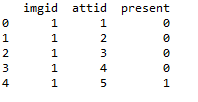
\includegraphics[width=10cm]{figures/1174077/3/9.png}}
\caption{Hasil 4 Bagian 2}
\label{labelgambar}
\end{figure}

\item Pada output berikutnya akan menampilkan jumlah kolom dan baris dari DataFrame variable imgatt.
\lstinputlisting[firstline=45, lastline=45]{src/1174077/3/Praktek.py}
\begin{figure}[H]
\centerline{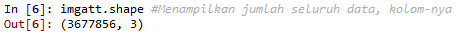
\includegraphics[width=10cm]{figures/1174077/3/10.png}}
\caption{Hasil 4 Bagian 3}
\label{labelgambar}
\end{figure}

\item Variabel imgatt2 telah menggunakan fungsi yang bernama pivot agar mengubah kolom jadi baris dan sebaliknya dari DataFrame imgatt sebelumnya.
\lstinputlisting[firstline=48, lastline=48]{src/1174077/3/Praktek.py}
\begin{figure}[H]
\centerline{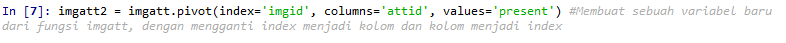
\includegraphics[width=10cm]{figures/1174077/3/11.png}}
\caption{Hasil 4 Bagian 4}
\label{labelgambar}
\end{figure}

\item Variabel imgatt2 head berfungsi untuk mengembalikan value teratas pada DataFrame imgatt2.
\lstinputlisting[firstline=51, lastline=51]{src/1174077/3/Praktek.py}
\begin{figure}[H]
\centerline{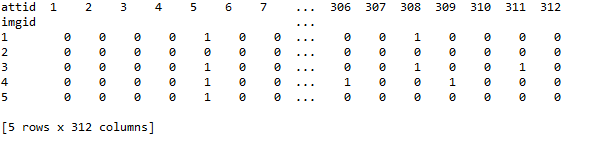
\includegraphics[width=10cm]{figures/1174077/3/12.png}}
\caption{Hasil 4 Bagian 5}
\label{labelgambar}
\end{figure}

\item Menghasilkan jumlah kolom dan baris pada DataFrame imgatt2.
\lstinputlisting[firstline=54, lastline=54]{src/1174077/3/Praktek.py}
\begin{figure}[H]
\centerline{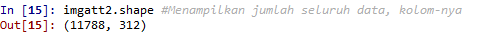
\includegraphics[width=10cm]{figures/1174077/3/13.png}}
\caption{Hasil 4 Bagian 6}
\label{labelgambar}
\end{figure}

\item Menunjukkan dalam melakukan pivot yang mana imgid menjadi sebuah index yang unik.
\lstinputlisting[firstline=57, lastline=60]{src/1174077/3/Praktek.py}
\begin{figure}[H]
\centerline{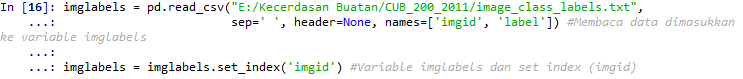
\includegraphics[width=10cm]{figures/1174077/3/14.png}}
\caption{Hasil 4 Bagian 7}
\label{labelgambar}
\end{figure}

\item Akan melakukan load jawabannya yang berisi apakah burung tersebut termasuk spesies yang mana. Kolom tersebut yaitu imgid dan label.
\lstinputlisting[firstline=68, lastline=68]{src/1174077/3/Praktek.py}
\begin{figure}[H]
\centerline{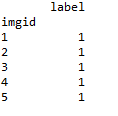
\includegraphics[width=10cm]{figures/1174077/3/15.png}}
\caption{Hasil 4 Bagian 8}
\label{labelgambar}
\end{figure}

\item Menunjukkan bahwa jumlah baris sebanyak 11788 dan kolom 1 yang dimana kolom tersebut adalah jenis spesies pada burung.
\lstinputlisting[firstline=71, lastline=71]{src/1174077/3/Praktek.py}
\begin{figure}[H]
\centerline{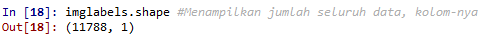
\includegraphics[width=10cm]{figures/1174077/3/16.png}}
\caption{Hasil 4 Bagian 9}
\label{labelgambar}
\end{figure}

\item Melakukan join antara imgatt2 dengan imglabels dikarenakan memiliki isi yang sama sehingga akan mendapatkan sebuah data ciri-ciri dan data jawaban sehingga bisa dikategorikan sebagai supervised learning.
\lstinputlisting[firstline=74, lastline=75]{src/1174077/3/Praktek.py}
\begin{figure}[H]
\centerline{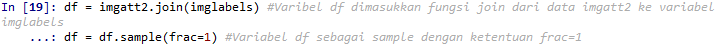
\includegraphics[width=10cm]{figures/1174077/3/17.png}}
\caption{Hasil 4 Bagian 10}
\label{labelgambar}
\end{figure}

\item Melakukan drop pada label yang ada didepan dan akan menggunakan label yang baru di joinkan.
\lstinputlisting[firstline=78, lastline=79]{src/1174077/3/Praktek.py}
\begin{figure}[H]
\centerline{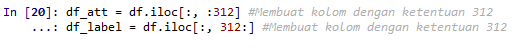
\includegraphics[width=10cm]{figures/1174077/3/18.png}}
\caption{Hasil 4 Bagian 11}
\label{labelgambar}
\end{figure}

\item Mengecek isi 5 data teratas pada df\_att.
\lstinputlisting[firstline=82, lastline=82]{src/1174077/3/Praktek.py}
\begin{figure}[H]
\centerline{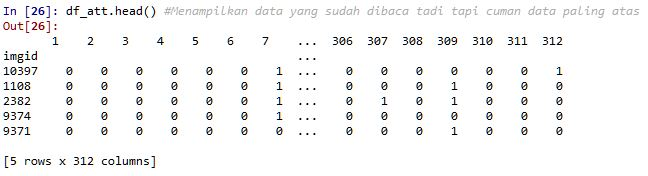
\includegraphics[width=10cm]{figures/1174077/3/35.png}}
\caption{Hasil 4 Bagian 12}
\label{labelgambar}
\end{figure}

\item Mengecek isi data teratas dari df\_label.
\lstinputlisting[firstline=85, lastline=85]{src/1174077/3/Praktek.py}
\begin{figure}[H]
\centerline{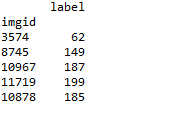
\includegraphics[width=10cm]{figures/1174077/3/19.png}}
\caption{Hasil 4 Bagian 13}
\label{labelgambar}
\end{figure}

\item Membagi 8000 row pertama menjadi data training dan sisanya adalah data testing.
\lstinputlisting[firstline=88, lastline=94]{src/1174077/3/Praktek.py}
\begin{figure}[H]
\centerline{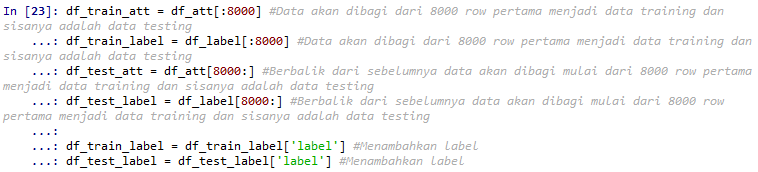
\includegraphics[width=10cm]{figures/1174077/3/20.png}}
\caption{Hasil 4 Bagian 14}
\label{labelgambar}
\end{figure}

\item Pemanggilan class RandomForestClassifier. Dimana artinya menunjukkan banyak kolom pada setiap tree adalah 50.
\lstinputlisting[firstline=97, lastline=98]{src/1174077/3/Praktek.py}
\begin{figure}[H]
\centerline{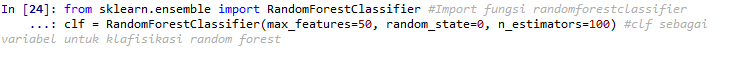
\includegraphics[width=10cm]{figures/1174077/3/21.png}}
\caption{Hasil 4 Bagian 15}
\label{labelgambar}
\end{figure}

\item Menunjukkan hasil prediksi dari Random Forest.
\lstinputlisting[firstline=101, lastline=101]{src/1174077/3/Praktek.py}
\begin{figure}[H]
\centerline{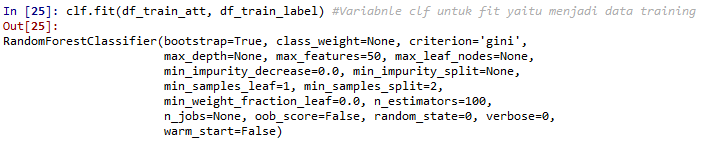
\includegraphics[width=10cm]{figures/1174077/3/22.png}}
\caption{Hasil 4 Bagian 16}
\label{labelgambar}
\end{figure}

\item Menampilkan besaran akurasi dari prediksi pada Random Forest yang merupakan score perolehan klarifikasi.
\lstinputlisting[firstline=104, lastline=104]{src/1174077/3/Praktek.py}
\begin{figure}[H]
\centerline{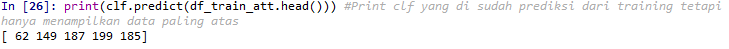
\includegraphics[width=10cm]{figures/1174077/3/23.png}}
\caption{Hasil 4 Bagian 17}
\label{labelgambar}
\end{figure}

\item Menampilkan besaran akurasi dari prediksi pada Random Forest yang merupakan score perolehan klarifikasi.
\lstinputlisting[firstline=107, lastline=107]{src/1174077/3/Praktek.py}
\begin{figure}[H]
\centerline{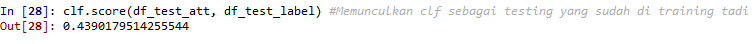
\includegraphics[width=10cm]{figures/1174077/3/24.png}}
\caption{Hasil 4 Bagian 18}
\label{labelgambar}
\end{figure}
\end{itemize}

\subsubsection{Nomor 5}
\hfill\break
\lstinputlisting[firstline=112, lastline=114]{src/1174077/3/Praktek.py}
\begin{figure}[H]
\centerline{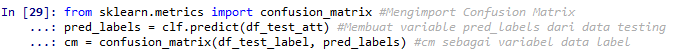
\includegraphics[width=10cm]{figures/1174077/3/25.png}}
\caption{Hasil 5 Bagian 1}
\label{labelgambar}
\end{figure}

\lstinputlisting[firstline=117, lastline=117]{src/1174077/3/Praktek.py}
\begin{figure}[H]
\centerline{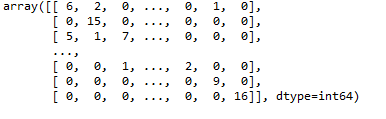
\includegraphics[width=10cm]{figures/1174077/3/26.png}}
\caption{Hasil 5 Bagian 2}
\label{labelgambar}
\end{figure}

\lstinputlisting[firstline=120, lastline=147]{src/1174077/3/Praktek.py}
\begin{figure}[H]
\centerline{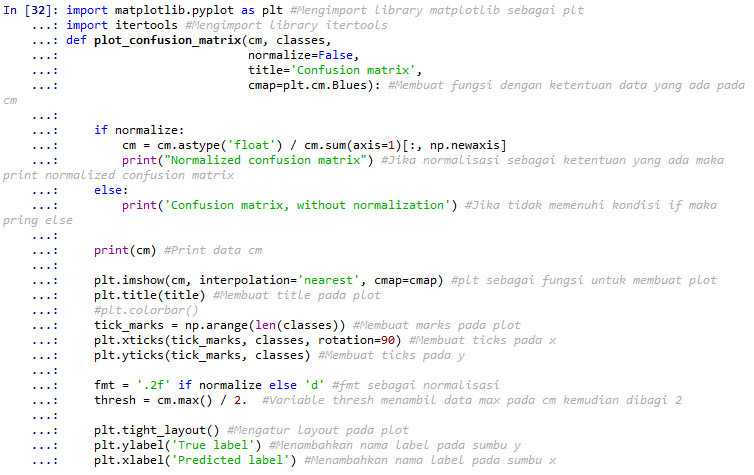
\includegraphics[width=10cm]{figures/1174077/3/27.png}}
\caption{Hasil 5 Bagian 3}
\label{labelgambar}
\end{figure}

\lstinputlisting[firstline=151, lastline=154]{src/1174077/3/Praktek.py}
\begin{figure}[H]
\centerline{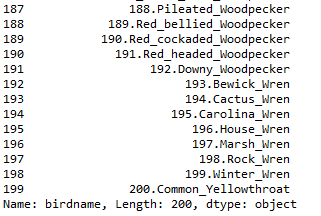
\includegraphics[width=10cm]{figures/1174077/3/28.png}}
\caption{Hasil 5 Bagian 4}
\label{labelgambar}
\end{figure}

\lstinputlisting[firstline=158, lastline=163]{src/1174077/3/Praktek.py}
\begin{figure}[H]
\centerline{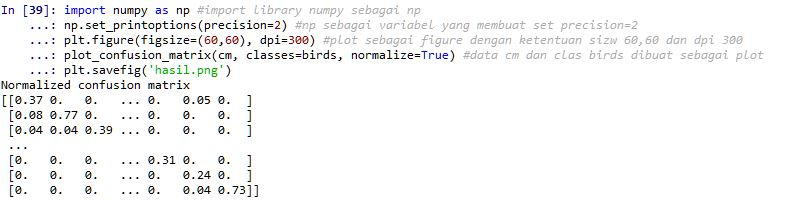
\includegraphics[width=10cm]{figures/1174077/3/36.png}}
\caption{Hasil 5 Bagian 5}
\label{labelgambar}
\end{figure}

\begin{figure}[H]
\centerline{\includegraphics[width=10cm]{figures/1174077/3/hasil.png}}
\caption{Plot Hasil 5 Bagian 5}
\label{labelgambar}
\end{figure}

\subsubsection{Nomor 6}
\hfill\break
\lstinputlisting[firstline=168, lastline=171]{src/1174077/3/Praktek.py}
\begin{figure}[H]
\centerline{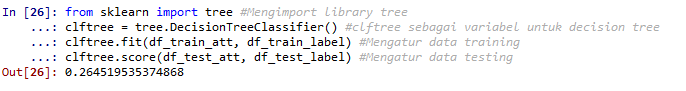
\includegraphics[width=10cm]{figures/1174077/3/29.png}}
\caption{Hasil 6 Bagian 1}
\label{labelgambar}
\end{figure}

\lstinputlisting[firstline=174, lastline=177]{src/1174077/3/Praktek.py}
\begin{figure}[H]
\centerline{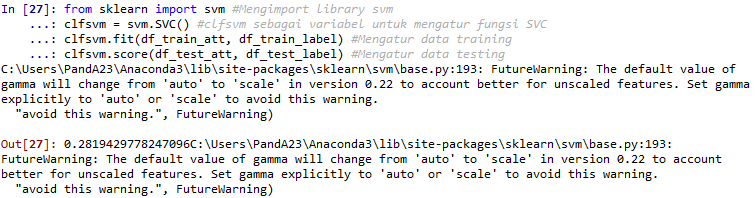
\includegraphics[width=10cm]{figures/1174077/3/30.png}}
\caption{Hasil 6 Bagian 2}
\label{labelgambar}
\end{figure}

\subsubsection{Nomor 7}
\hfill\break
\lstinputlisting[firstline=180, lastline=182]{src/1174077/3/Praktek.py}
\begin{figure}[H]
\centerline{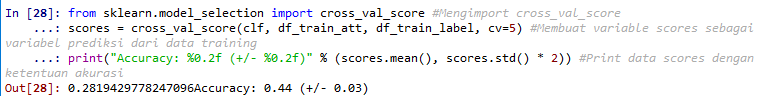
\includegraphics[width=10cm]{figures/1174077/3/31.png}}
\caption{Hasil 7 Bagian 1}
\label{labelgambar}
\end{figure}

\lstinputlisting[firstline=185, lastline=186]{src/1174077/3/Praktek.py}
\begin{figure}[H]
\centerline{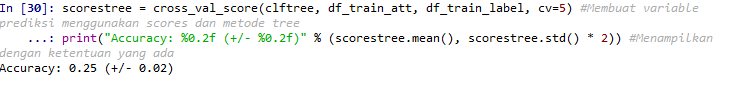
\includegraphics[width=10cm]{figures/1174077/3/32.png}}
\caption{Hasil 7 Bagian 2}
\label{labelgambar}
\end{figure}

\lstinputlisting[firstline=189, lastline=190]{src/1174077/3/Praktek.py}
\begin{figure}[H]
\centerline{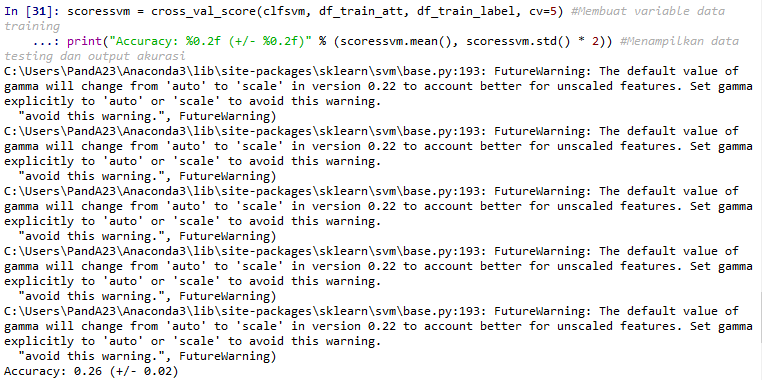
\includegraphics[width=10cm]{figures/1174077/3/33.png}}
\caption{Hasil 7 Bagian 3}
\label{labelgambar}
\end{figure}

\subsubsection{Nomor 8}
\hfill\break
\lstinputlisting[firstline=193, lastline=208]{src/1174077/3/Praktek.py}
\begin{figure}[H]
\centerline{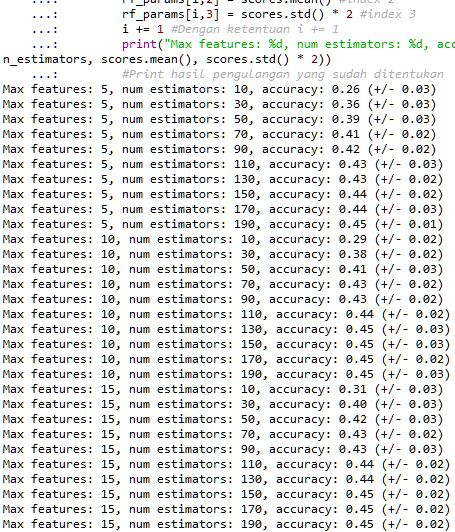
\includegraphics[width=10cm]{figures/1174077/3/37.png}}
\caption{Hasil 8 Bagian 1}
\label{labelgambar}
\end{figure}
\begin{figure}[H]
\centerline{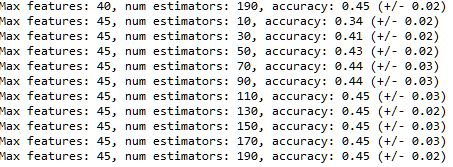
\includegraphics[width=10cm]{figures/1174077/3/38.png}}
\caption{Hasil 8 Bagian 1 Akhir kode}
\label{labelgambar}
\end{figure}

\lstinputlisting[firstline=210, lastline=224]{src/1174077/3/Praktek.py}
\begin{figure}[H]
\centerline{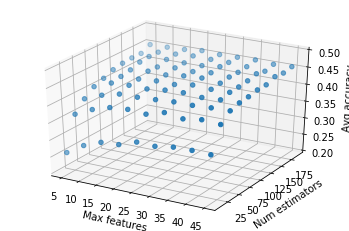
\includegraphics[width=10cm]{figures/1174077/3/39.png}}
\caption{Hasil 8 Bagian 2}
\label{labelgambar}
\end{figure}



\subsection{Penanganan Error}
\begin{enumerate}
	\item ScreenShoot Error
	\begin{figure}[H]
		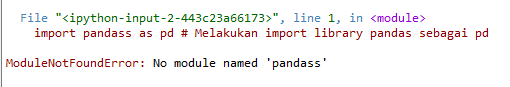
\includegraphics[width=4cm]{figures/1174077/3/error.png}
		\centering
		\caption{NoModuleFoundError}
	\end{figure}
	\item Tuliskan Kode Error dan Jenis Error
	\begin{itemize}
		\item NoModuleFoundError
	\end{itemize}
	\item Cara Penangan Error
	\begin{itemize}
		\item NoModuleFoundError
		\hfill\break
		Penulisan nama modul harus sesuai atau menginstall module yang diinginkan
	\end{itemize}
\end{enumerate}


\subsection{Bukti Tidak Plagiat}
\hfill\\
\begin{figure}[H]
\centerline{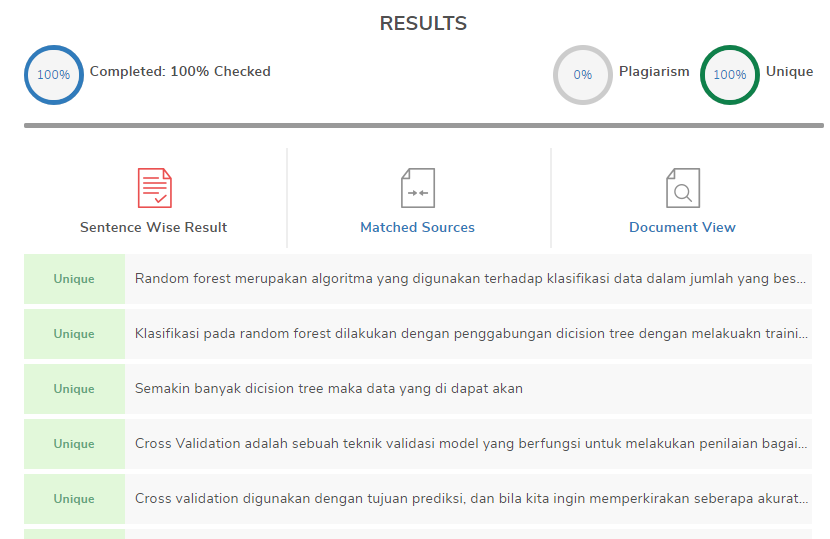
\includegraphics[width=10cm]{figures/1174077/3/plagiat.png}}
\caption{Bukti Tidak Plagiat}
\label{labelgambar}
\end{figure}